\chapter{Servidor de treball}\label{ch:server-description}

El procés de desenvolupament s’ha dut a terme emprant un servidor preparat pels directors del projecte, amb les següents característiques:

\begin{itemize}
    \item \textbf{Processador:}
    \begin{itemize}
        \item quatre cores
    \end{itemize}
    \item \textbf{Emmagatzemament:}
    \begin{itemize}
        \item 16 GB de disc de sistema.
        \item 256 GB de disc SSD per dades.
    \end{itemize}
\end{itemize}

\noindent
Aquest disposa de dos usuaris, \textit{tfe}, per l’ús diari, i un altre, amb privilegis d’administrador, \textit{root}, en cas que es necessitin aquests.
L’accés es realitza a través de l’usuari tfe, utilitzant una connexió \gls{ssh}:

\begin{verbatim}
    $ ssh tfe@ostia.epsevg.upc.edu
\end{verbatim}

\noindent
Les tasques principals realitzades són:

\begin{itemize}
    \item Desenvolupament del codi d’\gls{OSTIA}, utilitzant el sistema de control de versions git.
    \item Anàlisis dels \textit{\gls{log}s} d’\gls{UPCommons}, amb registres des del 2006 fins al 2023.
    \item Processament i abocament dels \textit{\gls{log}s} a la base de dades InfluxDB, ubicada al mateix servidor.
    \item Descàrrega de totes les metadades del servidor \gls{OAI} sbivdev1.
    \item Anàlisis, processament i abocament de les metadades a una base de dades \textit{MongoDB}.
    \item Anàlisi del conjunt de les dades, amb el suport l’eina \textit{Grafana}.
\end{itemize}

\clearpage

\section*{Configuració}\label{sec:server-configuration}

Els principals serveis utilitzats durant la realització del projecte han sigut:

\begin{itemize}
    \item \textbf{InfluxDB}
    \begin{itemize}
        \item Base de dades on hem emmagatzemat els \textit{\gls{log}s}.
        \item {
            Incorporem també el \textit{\gls{plugin}} d’InfluxDB anomenat Telegraf.
            Encara que el seu ús no és imperatiu pels nostres objectius, pot ser útil per recol·lectar dades del sistema.
        }
    \end{itemize}
    \item \textbf{MongoDB}
    \begin{itemize}
        \item Base de dades utilitzada per l’emmagatzematge de les metadades.
        \item El mateix servei no ofereix cap interfície gràfica, així perquè afegim el suport de mongodb-expres.
    \end{itemize}
    \item \textbf{Grafana}
    \begin{itemize}
        \item Principal eina d’observabilitat, emprada tant per l’anàlisi com per la visualització gràfica.
    \end{itemize}
\end{itemize}

\noindent
Per cadascun d’aquests serveis definirem un fitxer de configuració, que configurarà cada contenidor, que en aquest cas, són de tipus \textit{\gls{Docker}}. \\

\noindent
Com disposem de diverses aplicacions, la manera més senzilla és utilitzar el sistema per configurar i executar aplicacions multicontenidor per antonomàsia, que és \textit{\gls{docker-compose}}. \\

\noindent
Aquest fitxer acostuma a tenir aquesta estructura:

\begin{itemize}
    \item Definició del nom del servei.
    \item Imatge de \textit{\gls{Docker}} que es vol utilitzar.
    \item Els ports, definint el port de la màquina host i el del contenidor.
    \item El fitxer de configuració del servei.
    \item La xarxa interna del servei de \textit{\gls{Docker}} que adoptarà el servei.
    \item Altres opcions.
\end{itemize}

\clearpage

\noindent
A l'exemple següent es troba la configuració específica per la base de dades InfluxDB.

\begin{figure}[htbp]
    \centerline{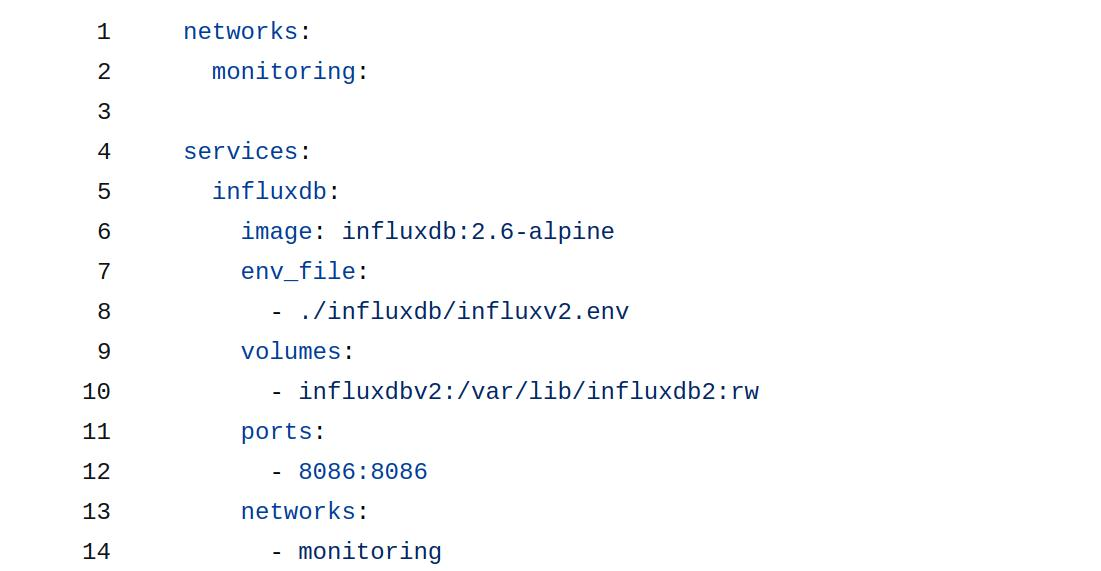
\includegraphics[width=\textwidth]{figures/docker-compose-influxdb}}
    \captionsetup{justification=centering}
    \caption{Configuració del servei d'InfluxDB. (\textbf{Font:} Repositori de codi del projecte.)}\label{fig:docker-compose-influxdb}
\end{figure}

\begin{tcolorbox}[colback=blue!5!white, colframe=blue!75!black, title=Fitxers de configuració]
    Habitualment aquests fitxers solen incloure credencials privades d'aquests serveis.
    Com a bona pràctica, afegeix el sufix \textit{.env} al fitxer i no el pugis a \textit{\gls{GitHub}}, omitin-lo mitjançant el fitxer \textit{.\gls{gitignore}}.
\end{tcolorbox}
\vspace{1em}

\noindent
Un cop definits tots els serveis, es procedeix amb la instal·lació.
La comanda següent descarrega les imatges de \textit{\gls{Docker}} en cas que aquestes no estiguin presents al sistema,
crea les xarxes virtuals pels contenidors i finalment, configura els serveis.

\begin{verbatim}
    $ docker compose up -d
\end{verbatim}

\begin{tcolorbox}[colback=red!5!white, colframe=red!75!black, title=Atenció]
    Aquesta comanda s'ha d'executar en el mateix directori on es troba el fitxer \textit{\gls{docker-compose}}.
\end{tcolorbox}

\clearpage

\section*{Accés als serveis}\label{sec:server-access}

\noindent
Per accedir als diferents serveis que es troben al servidor, utilitzarem un túnel \gls{ssh}~\cite{tunel-ssh}.
Aquest consisteix a xifrar tota comunicació entre client i servidor. \\

\noindent
Per exemple, el contingut de la interfície gràfica de Grafana, accessible a través del port tres mil del servidor,
serà accessible pel port tres mil de la màquina \textit{host} amb els següents passos:

\begin{verbatim}
    $ ssh -N -L localhost:3000:ostia.epsevg.upc.edu:3000 \
        tfe@ostia.epsevg.upc.edu
\end{verbatim}

\noindent
En un altre terminal:

\begin{verbatim}
    $ open https://localhost:3000
\end{verbatim}

\noindent \\
\section*{Instal·lació de software}\label{sec:software-installation}

El treball diari al servidor requereix de la instal·lació d'alguns paquets, alguns on la seva instal·lació és trivial utilitzant un gestor de paquets com \textit{\textit{apt}}, però d'altres en necessiten d'una instal·lació i configuració més curosa, com veurem amb \textit{\gls{Docker}}.

\noindent \\
Els paquets descarregats a través d'\textit{\gls{apt}} són els següents:

\begin{itemize}
    \item \texttt{git}: Comanda del sistema de control de versions \textit{\gls{git}} que permet fer un seguiment dels canvis en els fitxers de codi font.
    \item \texttt{tree}: Comanda que mostra el contingut d'un directori en forma d'arbre, mostrant la jerarquia de fitxers i carpetes de manera visual i estructurada.
    \item \texttt{python-venv}: Mòdul de \textit{Python} que crea entorns virtuals aïllats, permetent la instal·lació de paquets i dependències específiques per a un projecte sense afectar el sistema global.
    \item \texttt{pre-commit}: Mòdul per gestionar el codi abans de realitzar \textit{\gls{commit}s} a \textit{\gls{git}}, garantint que aquest compleixi amb les normes establertes.
\end{itemize}

\clearpage
\subsection*{\gls{Docker}}\label{subsec:docker-installation}

\begin{tcolorbox}[colback=red!5!white, colframe=red!75!black, title=sudo]
    La comanda \textit{sudo} és prescindible en cas d'estar utilitzant un usuari amb permisos d'administrador, com en el nostre cas, l'usuari \textit{root}.
\end{tcolorbox}

\noindent \\
Actualitzem la llista de paquets.
\begin{verbatim}
$ sudo apt-get update
\end{verbatim}

\noindent \\
Insta·lem les dependències requerides per \textit{\gls{Docker}}.
\begin{verbatim}
$ sudo apt-get install -y apt-transport-https ca-certificates \
    curl software-properties-common
\end{verbatim}

\noindent \\
Descarreguem, convertim a format binari i emmagatzemem la clau GPG oficial de \textit{\gls{Docker}}
\begin{verbatim}
$ curl -fsSL https://download.docker.com/linux/debian/gpg \
    | sudo gpg --dearmor \
    -o /usr/share/keyrings/docker-archive-keyring.gpg
\end{verbatim}

\noindent \\
Afegim a la llista de repositoris, el repositori de \textit{\gls{Docker}} corresponent a la nostra distribució.
\begin{verbatim}
$ echo "deb [arch=amd64 \
    signed-by\rightthreetimes=/usr/share/keyrings/docker-archive-keyring.gpg] \
    https://download.docker.com/linux/debian $(lsb_release -cs) stable" \
    | sudo tee /etc/apt/sources.list.d/docker.list > /dev/null\bullet
\end{verbatim}

\clearpage

\noindent \\
Instal·lem els paquets de \textit{\gls{Docker}}.
\begin{verbatim}
$ sudo apt install docker-ce docker-ce-cli containerd.io
\end{verbatim}

\noindent \\
Iniciem el servei.
\begin{verbatim}
$ sudo systemctl start docker
\end{verbatim}

\noindent \\
Habilitem que el servei s'iniciï automàticament cada vegada que es reinicia el sistema.
\begin{verbatim}
$ sudo systemctl enable docker
\end{verbatim}
